%%%%                %%%%
%%%% BASES TEÓRICAS %%%%
%%%%                %%%%

\chapter{Bases teóricas}
\label{chap:bases-teoricas}

\lettrine{E}l objetivo de este capítulo es sentar las bases tecnológicas y teóricas sobre las que se ha llevado a cabo el proyecto. En particular, se expone de qué manera se consiguen las coordenadas de las palabras y qué tecnologías intervienen para la obtención de la salida en formato estructurado.

Las aplicaciones comerciales utilizan las ubicaciones para seleccionar contenidos relevantes. Lo habitual es que el usuario pueda seleccionar rectángulos sobre las páginas y los procesos de extracción y verificación únicamente tengan en cuenta estas áreas. Para poder hacer esto se necesitan las localizaciones de las palabras, pares clave-valor, tablas, etc. Entre los PDF manejados para la elaboración de este trabajo hay dos categorías importantes: aquellos que tienen texto extraíble directamente y aquellos donde cada página es una imagen. El primer caso es el habitual en los PDF generados con procesadores de textos u otros software. Se puede comprobar fácilmente si un PDF contiene texto directamente extraíble abriendo el documento con un visor y realizando la selección con el ratón. Si es el caso, se puede evitar hacer OCR del documento y obtener una versión sin errores del texto.

\section{Software para la manipulación de PDF}

Existen librerías y también aplicaciones capaces de manipular ficheros PDF para extraer texto, imágenes, reordenar páginas y otras muchas posibilidades. Para los objetivos del proyecto, sería necesaria una herramienta capaz de extraer el texto pero también sus coordenadas sobre el documento. Se revisaron varias alternativas, como PDFBox \footnote{https://pdfbox.apache.org/}, Win2PDF \footnote{https://www.win2pdf.com/doc/command-line-extract-text-pdf.html}, ebook-convert \footnote{https://manual.calibre-ebook.com/es/generated/es/ebook-convert.html}, que forma parte de la aplicación Calibre, y pdftotext \footnote{https://poppler.freedesktop.org/}. Únicamente esta última ofrece la posibilidad de generar las localizaciones necesarias si se solicitan con el parámetro \verb|-bbox|. La salida es en formato XHTML.

Una limitación común en todas estas utilidades consiste en no respetar la disposición del texto, tal como aparece en el documento original. Esto implica que algunos elementos pueden aparecer antes que otros en la información extraída. Otro problema es que hay palabras que aparecen con caracteres intermedios, espacios, por ejemplo, que no se ven en el PDF. Estos problemas se derivan del propio funcionamiento del formato PDF.

\section{El formato PDF}

PDF es un formato digital para la creación de documentos. Fue introducido por Adobe Systems en 1993. En los siguientes años, el uso de este formato se extendió por toda la sociedad, tanto en el ámbito público como en el privado. En el año 2008, la ISO publicó el estándar 32000-1, tomando como base especificación de PDF en su versión 1.7, creada y liberada por Adobe. Posteriormente se publicó la versión 2.0 como ISO 32000-2 en el año 2017 y más recientemente una actualización en el año 2020. PDF es un modelo de representación de imágenes que deriva del lenguaje PostScript, también desarrollado por Adobe. En PDF, el modelo de imagen admite gráficos y texto de forma independiente al dispositivo de salida.

TODO Considerar si añadir más información de PostScript.

\subsection{Estructura de un PDF}

Un PDF no es un fichero de texto, es un fichero binario de 8 bits con una estructura interna determinada. Sus elementos básicos son los objetos. Cualquier información que se visualice en el documento existirá realmente como un objeto dentro del fichero. Estos objetos están serializados dentro del fichero y pueden ser de alguno de los siguientes nueve tipos:

\begin{enumerate}
    \item Null: se utiliza para indicar la ausencia de un valor.
    \item Boolean: indica los valores de verdad true o false.
    \item Integer: representa valores enteros. Puede aparecer como \verb|1|, \verb|+2|, \verb|-100|.
    \item Real: representa valores decimales y puede aparecer como \verb|0,05|, \verb|.25|, \verb|-3,1415|.
    \item Name: son secuencias únicas dentro del fichero, comienzan con una barra. Por ejemplo: \verb|/Type|, \verb|/ThisIsName|.
    \item String: puede ser de 4 tipos:
    \begin{itemize}
        \item ASCII: bytes codificados en ASCII.
        \item PDFDocEncoded: bytes codificados con la codificación PDFDocEncoding.
        \item Text: bytes codificados en PDFDocEncoding o UTF-16BE.
        \item Date: utilizado para fechas. Se codifican en ASCII con el patrón determinado. \footnote{D:YYYYMMDDHHmmSSOHH’mm}.
    \end{itemize}
    \item Array: es una colección heterogénea de objetos. Se escriben entre corchetes: \verb|[ 0 20 (E) ]|.
    \item Dictionary: es una tabla asociativa que contiene pares clave/valor. Pueden contener valores anidados y es utilizado para crear la jerarquía de todos los objetos del documento. Para indicar el comienzo y fin se utilizan los símbolos \verb|<<| y \verb|>>|. Las claves se indican con valores de tipo name.
    \item Streams: son secuencias de bytes de 8 bits sin límite de tamaño. Son utilizados para almacenar cualquier información binaria, por ejemplo imágenes, ficheros JSON o tipografías. Los stream tienen como preámbulo un diccionario de propiedades del stream. Este diccionario siempre debe contener, al menos, la clave \verb|/Length| que indica en bytes el tamaño del stream. Otra clave importante es \verb|/Filter|. \verb|/Filter| indica que la información está comprimida o codificada. Las imágenes se suelen codificar como DCTDecode o JPXDe que son versiones diferentes del formato JPEG. Para otro tipo de datos está disponible el algoritmo FlateDecode, similar a  DEFLATE, el mismo utilizado en los ficheros ZIP.
\end{enumerate}

Los objetos presentados hasta el momento son los objetos directos. Los objetos directos tienen el valor almacenado en el propio objeto. También existen los objetos indirectos que se referencian indirectamente y el consumidor tiene que saltar a otra posición en el fichero. Los objetos indirectos tienen un identificador único dentro del fichero. Las referencias son de la forma: \verb|/ObjIndirecto  5 0 R|.

\subsection{Estructura de un fichero PDF}

La estructura de un fichero está dividida en cuatro partes, header, body, cross-reference table y trailer. El header tiene al menos dos líneas. La primera se utiliza para indicar que el fichero es un PDF y la versión del estándar que le corresponde. La segunda es simplemente un separador: \verb|%%EOF|. El trailer es un objeto de tipo diccionario. Contiene claves y valores que aportan información a nivel de documento. Hay dos claves especialmente importantes, /Size que indica el número de entradas de la Cross-reference table y /Root que apunta al objeto que contiene el comienzo del Catálogo. El body contiene el objeto del Catálogo y todos los demás objetos que conforman el contenido del fichero PDF. La Cross-Reference Table es un índice de todos los objetos indirectos del PDF. Se utiliza para implementar la navegación sobre el fichero. Contiene la información necesaria para poder realizar saltos a la posición donde se encuentra el objeto que se quiere leer. La versión tradicional tiene tres columnas y la secuencia de entradas hace referencia al número del objeto buscado. En el ejemplo, para encontrar el objeto 2, tercera entrada, hay que saltar hasta el byte 32800:

0000000000 65535 f
0000000009 00000 n
0000032800 00000 n
0000000203 00000 n
0000000298 00000 n
0000008654 00000 n
0000000335 00000 n

TODO Considerar hablar del catálogo o dejarlo para la parte de implementación.

%%%%%

\section{Información de coordenadas en documentos}

La base de este proyecto consiste en utilizar las coordenadas físicas de los textos existentes en los documentos. Dado que los PDF pueden contener una representación textual o simplemente imágenes por cada página, es necesario encontrar una solución aplicable a cada caso y que permita un tratamiento homogéneo en los sucesivos pasos.

\subsection{El microformato hOCR y otras alternativas}

HOCR es un microformato para la representación de la información de salida del proceso OCR. Los microformatos permiten dotar de datos estructurados a 

\subsection{Pdftotext e información de bounding box}

\verb|pdftotext| es una herramienta que permite extraer el texto contenido en un PDF. Existen otras herramientas similares, por ejemplo Apache PDFBox \cite{the_apache_software_foundation_apache_nodate}, pero durante el desarrollo \verb|pdftotext| fue la que mostró los resultados más útiles para los objetivos del proyecto. La implementación original de esta utilidad fue realizada por Glyph \& Cog \cite{glyph__cog_llc_glyph_nodate-1} junto con otras herramientas para tratamiento del formato PDF. En el año 2005 nace la librería Poppler a partir del \emph{fork} de la versión 3.0.3 del visor de \verb|xpdf| \cite{kristian_hogsberg_poppler_2012}. La implementación de Poppler está disponible por defecto en las principales distribuciones Linux. Además del extractor de texto, el proyecto tienen otras utilidades para tratamiento de PDF, por ejemplo, separación y unión de páginas, obtención de imágenes, etc.

La salida con la información de coordenadas, o bounding box, además del texto existe gracias a una aportación al proyecto del año 2010 de Kenneth Berland \cite{kenneth_berland_poppler_2010}. La información se proporciona en formato XHTML y se identifican \emph{tags} para bloques, lineas y palabras. En cada uno se informa de la localización del rectángulo que engloba al elemento con cuatro valores: \emph{xMin}, \emph{xMax}, \emph{yMin}, \emph{yMax}.

%% Incluir imagen del rectángulo
\begin{figure}[hp!]
	\centering
	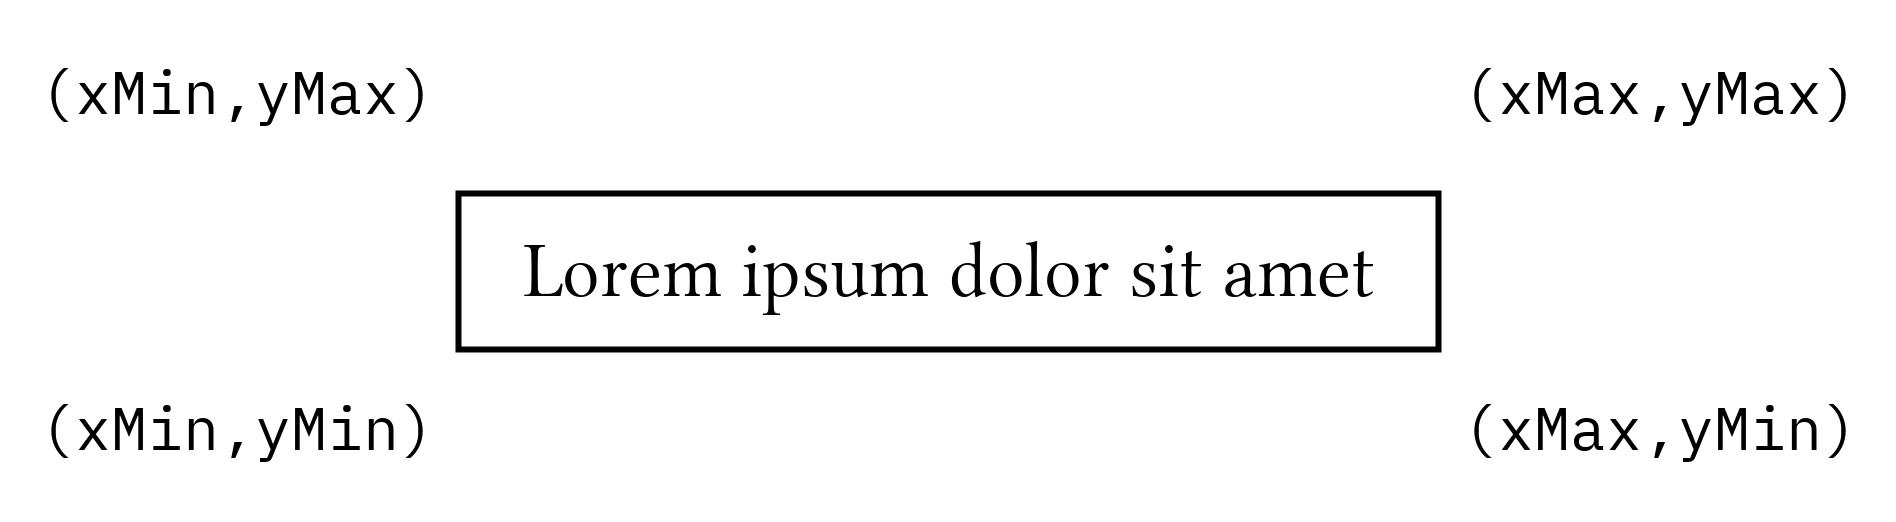
\includegraphics[width=0.75\textwidth]{imaxes/c-fundamentos-techno/correspondencia-coordenadas-bounding.png}
	\caption{Correspondencia de las coordenadas en una bounding box}
	\label{fig:bounding-box}
\end{figure}

\section{Reconocimiento Óptico de Caracteres}

Existen numerosas herramientas para llevar a cabo Reconocimiento Óptico de Caracteres. Entre ellas destaca Tesseract. Tesseract es un \emph{engine} de código abierto y desarrollado inicialmente por Hewlett Packard entre los años 1985 y 1995. Después de un periodo sin actividad, en el 2006 el proyecto fue recuperado por Google, que lo mantiene desde entonces.

Hoy en día tiene soporte para más de cien idiomas y la red neuronal que utiliza \footnote{Desde la versión 4, Tesseract utiliza una red LSTM. Esta es una red neuronal de tipo recurrente o RNN} puede ser entrenada para casos específicos si fuese necesario. Existe una amplia documentación en la web oficial, además, numerosos tutoriales en la red permiten familiarizarse con la herramienta al tratarse de un proyecto bien conocido y de larga trayectoria.

Se puede obtener como salida el texto reconocido y también la información de las coordenada, sobre el documento, de las palabras detectadas. Esta información resulta fundamental para poder aplicar las plantillas utilizadas este proyecto.

\section{Detección de líneas en las tablas}

La Transformada de Hough es una técnica de visión por computador utilizada para detectar figuras parametrizables, tales como líneas o círculos. El algoritmo parte de una imagen binaria que representa los bordes encontrados por una detector de bordes. A continuación se calculan todas las posibles líneas que podrían pasar por cada punto y se lleva a cabo una votación. Se seleccionan las líneas más votadas, entre todas las detectadas.

Este algoritmo proporciona una manera automática de localizar los bordes entre líneas de las tablas de muchos documentos y evita la necesidad de incorporar dicha información a las plantillas de forma manual. Se utiliza la implementación incluida en la librería OpenCV.

\section{Análisis léxico y sintáctico}

Flex y Bison son dos herramientas utilizadas en conjunto para construir analizadores sintácticos. ¿Qué es un analizador sintáctico?

La primera se utiliza para crear escáneres y la segunda para generar parsers. Ambas utilizan como entrada unos ficheros que definen las reglas válidas.

\section{GNU Make}

GNU Make es una herramienta que permite automatizar transformaciones sobre ficheros. \verb|make| es capaz de construir ejecutables a partir del código fuente de un proyecto. Para ello utiliza un fichero \verb|makefile| que contiene todas las reglas necesarias.

\section{Ansible}

\section{Docker}

%% Valorar si mencionar otras herramientas como:
% Extracción de texto: , pdftotext
% Pretty print de JSON: jq
